\documentclass{article}
\usepackage[utf8]{inputenc}
\usepackage{amsmath}
\usepackage{tcolorbox}
\usepackage{indentfirst}
\usepackage{graphicx}
\usepackage{minted}
\usepackage{float}
\usepackage [english]{babel}
\usepackage [autostyle, english = american]{csquotes}
\MakeOuterQuote{"}

\title{System on a Chip Class Report 5}
\author{Jordan D Edwards}
\date{October 2023}


\begin{document}
	
	\title{Class Report 5
		\\ \large{ELC 4396 System on a Chip}  }
	
	\author{Jordan Edwards \\ Baylor University} %the \\ symbols starts a new line
	\date{November 14, 2023}
	\maketitle
	
	\subsection*{Introduction}
	For this assignment, I used the I2C communication protocol to read from an onboard temperature sensor. This data was then displayed on the built-in seven-segment displays.
	
	
	\subsection*{Implementation}
	In Vivado, I was able to add in the I2C communication by adding it in to the appropriate slot and making the necessary wires travel out to the base file. On the software side, I utilized the sampler code as a base for getting the temperature and converting it to Celsius. From there, I multiplied it by 100 and stored it in an integer to eliminate further decimal places, treating this number a a fixed-point number. I then iterated through the number, output each digit individually. Finally, I placed a decimal point between the second and third digits from the right.
	
	\begin{figure}[H]
		\centering
		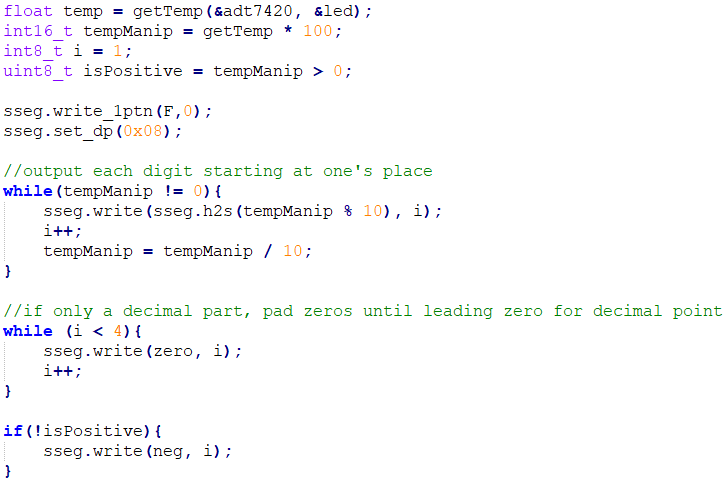
\includegraphics[width=\linewidth]{code}
		\caption{Display code}
		\label{fig:code}
	\end{figure}
	
	\subsection*{Results}
	I have yet to test this code as I do not currently have access to Vitis to compile or upload it.
\end{document}
